\documentclass{beamer}
\usetheme[pageofpages=of,% String used between the current page and the
                         % total page count.
          bullet=circle,% Use circles instead of squares for bullets.
          titleline=true,% Show a line below the frame title.
          alternativetitlepage=true,% Use the fancy title page.
       %   titlepagelogo=logo-polito,% Logo for the first page.
       %   watermark=watermark-polito,% Watermark used in every page.
       %   watermarkheight=100px,% Height of the watermark.
       %   watermarkheightmult=4,% The watermark image is 4 times bigger
                                % than watermarkheight.
          ]{Torino}

\setbeamertemplate{footline}{
  \begin{beamercolorbox}[wd=\paperwidth,ht=1ex,dp=1ex]{footline}
    \vspace{5pt} \hspace{1em} \insertframenumber/\inserttotalframenumber
  \end{beamercolorbox}
}

\author{Brendon J. Brewer}
\title{STATS 331 -- Introduction to Bayesian Statistics}
\institute{The University of Auckland}
\date{}


\linespread{1.3}
\usepackage{minted}
\usepackage[utf8]{inputenc}
\usepackage{dsfont}
\newcommand{\given}{\,|\,}

\begin{document}

\frame{\titlepage}

\begin{frame}
\begin{center}
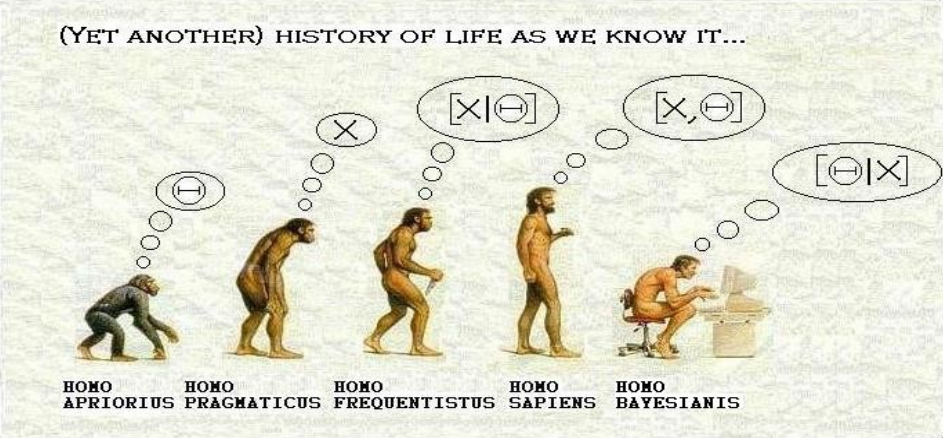
\includegraphics[width=0.9\textwidth]{images/history.png} \\
Credit: Unknown but maybe Bill Jeffreys?
\end{center}

\end{frame}


\begin{frame}

\begin{center}
Summarising Posterior Distributions
\end{center}

\end{frame}

\begin{frame}
\frametitle{The Posterior}
\begin{itemize}
\item In Bayesian statistics, posterior distributions form the complete answer
to the question ``what is known about $\theta$''? \pause
\item From the posterior distribution, you can calculate the probability of
anything else you might be interested in (e.g., predictions).
\end{itemize}

\end{frame}

\begin{frame}
\frametitle{Posterior Summaries}

\begin{itemize}
\item The posterior might be a complicated probability distribution, or it
might be simple, but in any case it is nice to be able to communicate what it
looks like to others. \pause
\item If we summarise with a `point estimate' (single number guess) or
an interval, then we have some things which are analogous to frequentist
estimators and confidence intervals.\pause
\item Posterior summaries are often analogous to simple summaries of datasets.
\end{itemize}

\end{frame}


\begin{frame}
\frametitle{Simple Summaries}
Here are some summaries which are common, and you might have already thought
of them. We often want to convey something about where the distribution is
centered and how wide it is.\pause

The posterior mean (expected value) and standard deviation are reasonable
choices for this in many cases.\pause

{\bf posterior mean $\pm$ posterior s.d.}
is approximately a 68\% credible interval
(we will see these later) if the posterior is approximately a normal/gaussian
distribution.

\end{frame}

\begin{frame}[fragile]
\frametitle{Computing Simple Summaries}
\begin{minted}{r}
# Posterior mean
post_mean = sum(theta*post)

# Variance and s.d.
post_var = sum((theta - post_mean)^2*post)
post_sd = sqrt(post_var)
\end{minted}
(These will change when we start using MCMC)

\end{frame}


\begin{frame}[fragile]
\frametitle{Example Posterior Distribution}
Remember our election polling example, with 6 successes out of 10 Bernoulli
trials. The posterior was a Beta$(7, 5)$ distribution.

\begin{center}
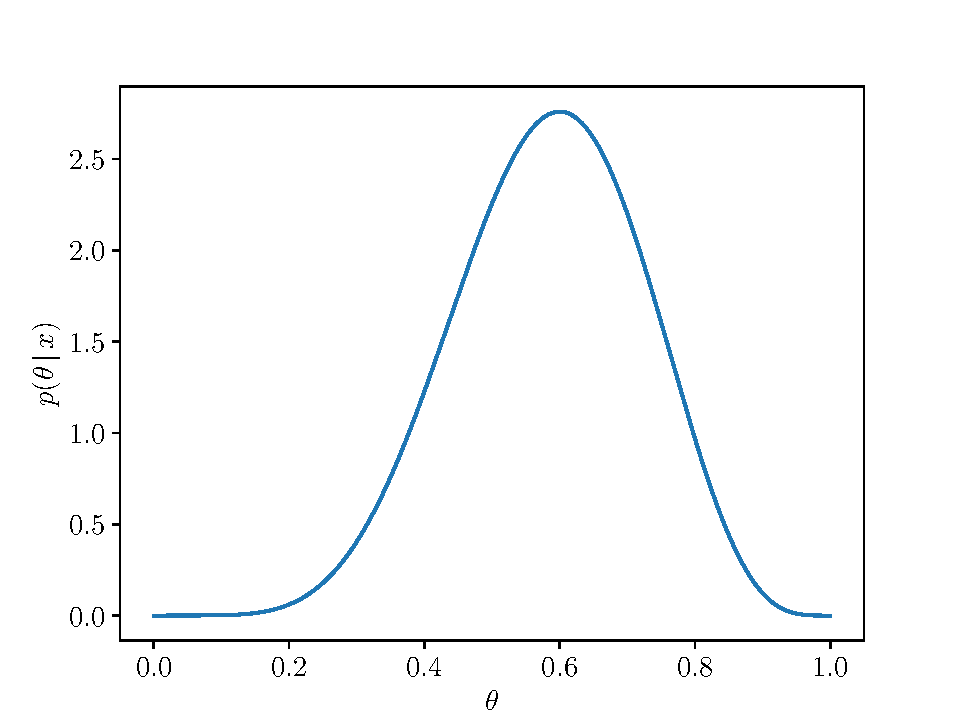
\includegraphics[width=0.65\textwidth]{images/beta_posterior.pdf}
\end{center}

\end{frame}


\begin{frame}[fragile]
\frametitle{Example Posterior Distribution}

The mean of this is 7/12 $\approx 0.583$ (as we saw when we did prediction)
and the s.d. is available analytically. We get
\begin{align}
\theta = 0.583 \pm 0.137.
\end{align}


\end{frame}


\begin{frame}
\frametitle{Other Options for Point Estimates}
The posterior mean is not the only option for presenting a point estimate.
We also have, for example, the posterior median or the posterior mode.\\[0.5em]\pause

Let's look at these for the election poll posterior distribution.
\end{frame}

\begin{frame}[fragile]
\frametitle{Computing Point Estimates (Grid Method)}

\begin{minted}{r}
# Mean
posterior_mean = sum(theta*post)
# Mode
highest_probability = max(post)
posterior_mode = theta[post == highest_probability]
# Median
F = cumsum(post)
dist = abs(F - 0.5)
posterior_median = theta[dist == min(dist)]
\end{minted}
(These will change when we learn MCMC)

\end{frame}



\begin{frame}
\frametitle{Three Options for Point Estimates}
\begin{center}
\includegraphics[width=0.6\textwidth]{images/point_estimates.pdf}
\end{center}

They are all close together, because the distribution is quite symmetric.
But this won't always be the case.

\end{frame}



\begin{frame}
\frametitle{Decision Theory}
When you are forced to make a choice, how do you make the {\em best} possible
choice?\\[0.7em]
\pause

{\em 
``You acted unwisely'', I cried, ``as you see
by the outcome''. He calmly eyed me:
``When choosing the course of my action'', said he, ``I had
not the outcome to guide me.'' -- Ambrose Bierce
}

\end{frame}


\begin{frame}
\frametitle{Decision Theory}
Our information is embodied in the posterior distribution,
which ought to contain the consequences of everything
known and relevant to the value of the parameters.
\pause

Some actions/decisions are {\bf probably} better than others,
and this can be formalised.
\end{frame}

\begin{frame}
\frametitle{Point Estimates}

\begin{itemize}
\item If we are inferring a parameter $\theta$ from data, we could
give a single number guess, which we call $\hat{\theta}$. \pause
\item In classical statistics, rules for producing these are called point
estimators. \pause
\item  In Bayesian, if we have to choose a single point estimate,
the value that we choose is a decision or an action. We
get the appropriate value of $\hat{\theta}$
from decision theory based on the posterior
distriution.
\end{itemize}

\end{frame}

\begin{frame}
\frametitle{Best Point Estimate}
\begin{itemize}
\item Obviously, the best possible choice for the value of $\hat{\theta}$ is to
set it equal to the true value of $\theta$.\pause
\item Since we don't know the true value, our definition of what it means to
be `best' needs to be modified.\pause
\item Be wary of anything in statistics that claims to be `optimal', because
there will always be qualifiers.
\end{itemize}
\end{frame}


\begin{frame}
\frametitle{Utility Function}
If the true value is $\theta$ and our estimate is $\hat{\theta}$, how good is
our estimate? We describe this with a {\bf utility function} $U(\hat{\theta}, \theta)$.
We want the value of $U$ to be high. \pause

Alternatively, with a minus sign, we can
define a {\bf loss function}, which we want to be low:
\begin{align}
L(\hat{\theta}, \theta) &= -U(\hat{\theta}, \theta).
\end{align}
\pause
In applications, $L$ and $U$ are sometimes dollar amounts!

\end{frame}


\begin{frame}
\frametitle{Three Loss Functions}
Here are three common choices for the loss function:

\begin{align}
L &= (\hat{\theta} - \theta)^2 \\
L &= |\hat{\theta} - \theta| \\
L &= \left\{
        \begin{array}{lr}
        0, & \hat{\theta} = \theta \\
        1, & \textnormal{otherwise.}
        \end{array}
        \right.
\end{align}

These are the quadratic loss, absolute loss, and all-or-nothing loss
respectively.
\end{frame}



\begin{frame}
\frametitle{Three Loss Functions}

\centering
\includegraphics[width=0.7\textwidth]{images/loss_functions.pdf}

\end{frame}

\begin{frame}
\frametitle{Loss Functions}
What do we do with the loss function? We can't minimise it because we don't
know $\theta$. Instead, we minimise the {\bf expected loss} according to the
posterior distribution.

\begin{align}
E\left[L(\hat{\theta}, \theta)\right]
    &= \int p(\theta \given x) L(\hat{\theta}, \theta) \, d\theta.
\end{align}

\end{frame}


\begin{frame}
\frametitle{Quadratic Loss Function}
If the loss function is quadratic, the posterior mean is the best estimate!

\begin{align}
\frac{d}{d\hat{\theta}}\mathds{E}\left[L(\hat{\theta}, \theta)\right] &=
\int p(\theta \given x)\frac{d}{d\hat{\theta}}(\hat{\theta} - \theta)^2 \, d\theta \\
&= \int p(\theta\given x)2(\hat{\theta} - \theta) \, d\theta
\end{align}
Setting this equal to zero and then solving for $\hat{\theta}$ gives the final
result:
\begin{align}
\hat{\theta} &= \int \theta p(\theta\given x) \, d\theta.
\end{align}


\end{frame}


\begin{frame}
\frametitle{Absolute Loss Function}
If the loss function is the absolute value form,
the posterior median is the best estimate!\pause

Proof: Beyond the scope of this course.
\end{frame}


\begin{frame}
\frametitle{Absolute Loss Function}
The posterior median has the nice property that it is invariant under
changes in parameterisation. For example, if $\phi = \log(\theta)$ then
the posterior median for $\phi$ corresponds to the posterior median for
$\theta$.

\end{frame}


\begin{frame}
\frametitle{All-or-Nothing Loss Function}
If the loss function is the all-or-nothing form,
the posterior mode is the best estimate!\pause

Proof: Beyond the scope of this course, but here's some intuition:
You need to be exactly right with your estimate, so you may as well
choose the value with the highest posterior probability.
\end{frame}


\begin{frame}
\frametitle{All-or-Nothing Loss Example}
\begin{itemize}
\item You are in a dark cave, being chased by a small, dangerous bat. You have
a gun.\pause
\item Based on the sounds you hear, you have a posterior distribution for the
direction to the bat.\pause
\item Since it matters that you hit the bat, and there is no reward for
merely being close, we have an all-or-nothing loss situation.\pause
\item Therefore, shoot at the posterior mode.
\end{itemize}


\end{frame}


\begin{frame}[fragile]
\frametitle{Credible Intervals}
\begin{verbatim}
                 |---------------------|
\end{verbatim}

\end{frame}


\begin{frame}[fragile]
\frametitle{Credible Intervals}
Credible intervals are like frequentist confidence intervals, but more sensible
(in my opinion). To compute them, find an interval that contains a certain
amount of posterior probability inside it, such as 95\%.

\end{frame}


\begin{frame}[fragile]
\frametitle{Computing Credible Intervals}
\begin{itemize}
\item To compute a credible interval in R, the calculation is very similar to the
posterior median. You find the point at which the cumulative probability
crosses (for instance) 2.5\% and 97.5\%.\pause
\item As with the posterior median, the method will be different once we
deal with MCMC instead of a grid.
\end{itemize}

\end{frame}



\begin{frame}[fragile]
\frametitle{Shifted Exponential Example}
\begin{itemize}
\item This example, due to Ed Jaynes, demonstrates that frequentist confidence intervals
and Bayesian credible intervals are {\bf not the same concept}.\pause
\item Often, the two types of intervals will give the same numerical result, so
many people do not realise they are conceptually different.
\end{itemize}

\end{frame}

\begin{frame}[fragile]
\frametitle{Shifted Exponential Example}
\begin{itemize}
\item New widgets are injected with a chemical that helps
them to function.\pause
\item Widgets are guaranteed to work for a certain duration. That duration is the
unknown parameter $\theta$.\pause
\item After $\theta$ time has passed, the widgets fail with a mean lifetime
of one year.
\end{itemize}

\end{frame}


\begin{frame}[fragile]
\frametitle{Shifted Exponential Example}
The sampling distribution for a single widget's lifetime, $x$, is given by
\begin{align}
p(x \given \theta) &= \left\{
    \begin{array}{lr}
    e^{\theta - x}, & x > \theta \\
    0,              & \textnormal{otherwise.}
    \end{array}
    \right.
\end{align}

\end{frame}


\begin{frame}[fragile]
\frametitle{Shifted Exponential Example: Sampling Distribution}
\centering
\includegraphics[width=0.7\textwidth]{images/shifted_exponential.pdf}

\end{frame}



\begin{frame}[fragile]
\frametitle{Shifted Exponential Example: Sampling Distribution}
In the example, the data consists of three values, so the sampling distribution
becomes
\begin{align}
p(x_1, x_2, x_3 \given \theta)
    &= \left\{
    \begin{array}{lr}
     \prod_{i=1}^3  e^{\theta - x_i}, & \textnormal{all }x\textnormal{s} > \theta \\
    0,              & \textnormal{otherwise.}
    \end{array}
    \right.
\end{align}

\pause

The observed values are $\boldsymbol{x} = \{12, 14, 16\}$.


\end{frame}


\begin{frame}[fragile]
\frametitle{Shifted Exponential Example: Likelihood Function}
If we plug in the observed data, we get the likelihood function.

\begin{align}
p(x_1, x_2, x_3 \given \theta)
    &= \left\{
    \begin{array}{lr}
    e^{3\theta - 42}, & \theta < 12\\
    0,              & \textnormal{otherwise.}
    \end{array}
    \right.
\end{align}
Importantly, {\bf the data completely rules out some values of} $\theta$.
\pause

For the prior, we can use $\theta \sim \textnormal{Uniform}(0, 20)$.
\end{frame}



\begin{frame}[fragile]
\frametitle{Computing the Result}
\begin{minted}{r}
theta = seq(0, 20, by=0.01)
prior = rep(1/length(theta), length(theta))
lik = exp(3*theta - 42)
lik[theta > 12] = 0
h = prior*lik
Z = sum(h)
post = h/Z
plot(theta, post, type="l")
\end{minted}

\end{frame}


\begin{frame}[fragile]
\frametitle{Shifted Exponential Example: Posterior Distribution}
\centering
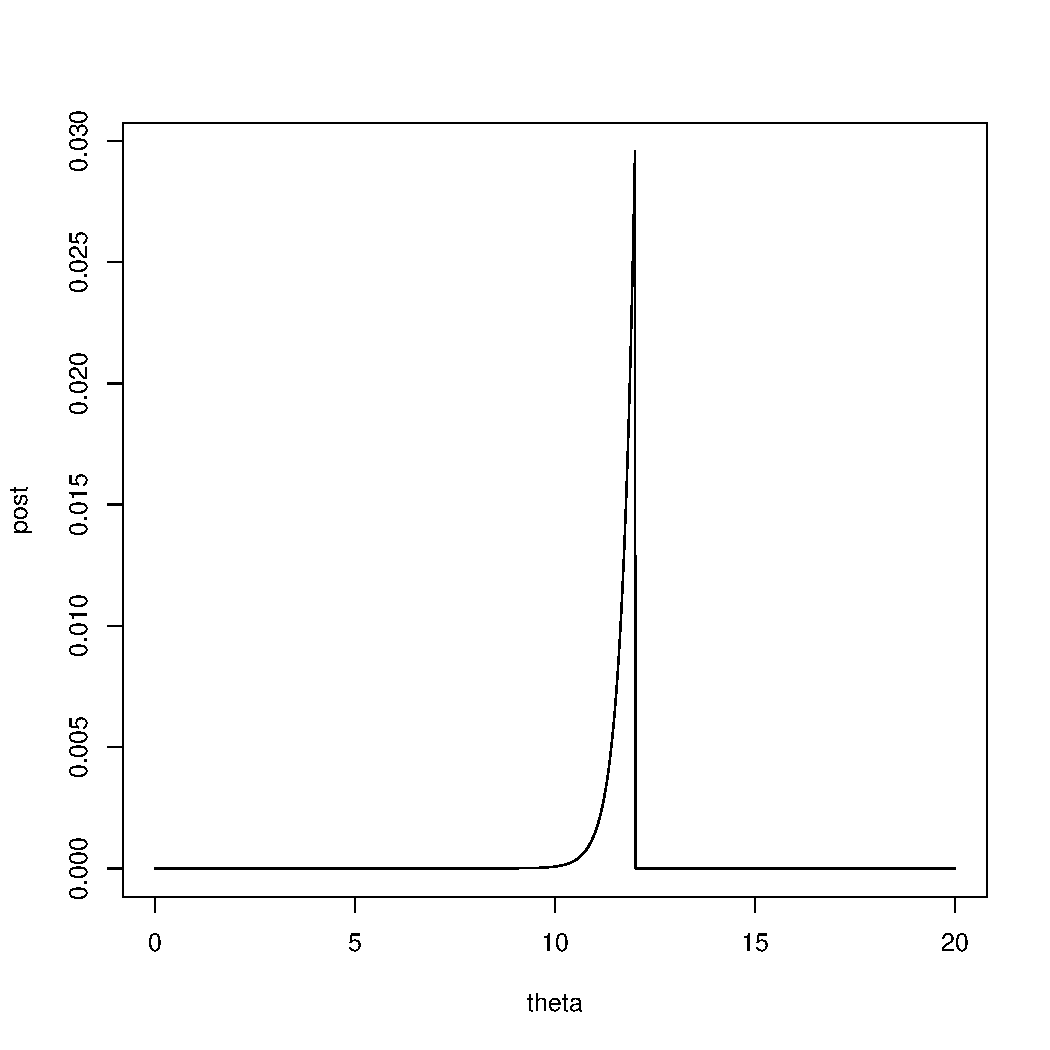
\includegraphics[width=0.6\textwidth]{images/widget_posterior.pdf}

\end{frame}


\begin{frame}[fragile]
\frametitle{90\% Credible Interval}

\begin{minted}{r}
F = cumsum(post)
dist = abs(F - 0.05)
left = theta[dist == min(dist)]
dist = abs(F - 0.95)
right = theta[dist == min(dist)]
\end{minted}
\pause

The result is $[11.00, 11.98]$, which seems sensible.
Now let's do a frequentist confidence interval.
\end{frame}


\begin{frame}[fragile]
\frametitle{Credible Intervals vs. Confidence Intervals}
Credible intervals are based on the posterior distribution.
\begin{align}
P(\theta \textnormal{ in interval} \given x)
    &= 0.95.
\end{align}

\pause

Confidence intervals are based on the sampling distribution.
\begin{align}
P(\theta \textnormal{ in interval} \given \theta)
    &= 0.95.
\end{align}

\end{frame}


\begin{frame}[fragile]
\frametitle{Widgets: Frequentist Estimator and Confidence Interval}
There are different estimators and confidence interval recipes you could use,
but here is one:

\begin{align}
\hat{\theta} = \frac{1}{N}\sum_{i=1}^N (x_i - 1) \\
[\hat{\theta} - 0.8529, \hat{\theta} + 0.8264]
\end{align}

\end{frame}


\begin{frame}[fragile]
\frametitle{Widgets: Verifying the Confidence Interval}
\footnotesize
\begin{minted}{r}
inside = 0
theta = 10
for(i in 1:1000000)
{
    x = theta - log(runif(3)) # Generate from shifted exponential
    theta_hat = mean(x - 1)
    left = theta_hat - 0.8529
    right = theta_hat + 0.8264
    if(theta > left && theta < right)
        inside = inside + 1
}
inside/1000000 # I got 0.89883
\end{minted}
\end{frame}


\begin{frame}
\frametitle{Widgets: Confidence Interval}
\begin{itemize}
\item We have verified that the interval contains the true value of $\theta$
`90\% of the time' (for 90\% of possible datasets). Now, let's apply it to our
actual dataset $\{12, 14, 16\}$. \pause
\item The confidence interval is $[12.1471, 13.8264]$. \pause
\item As a reminder, the credible interval was $[11.00, 11.98]$ --- so they are
different.
\end{itemize}

\end{frame}

\begin{frame}
\frametitle{Widgets: Confidence Interval}
Remember that, in the posterior distribution, all values of $\theta$
above 12 are completely ruled out. But that rules out the whole confidence
interval!

\pause

The problem is that, while the interval works for 90\% of data sets,
this data set is in the 10\% where it doesn't --- and we can tell that from the
data.
\end{frame}


\begin{frame}
\frametitle{Confidence Intervals}
\begin{itemize}
\item Other ways of making a confidence interval exist, and some of them might avoid
this particular problem.\pause
\item Different Bayesian credible intervals could be produced only by modifying the
prior distribution, and they would never have this particular problem.\pause
\item What is the question you really want to answer?
\end{itemize}

\end{frame}


\begin{frame}
\frametitle{Confidence Intervals and Credible Intervals}
\begin{itemize}
\item As mentioned earlier, often, the two types of intervals produce the same
numerical result, even though they are different concepts. \pause
\item This often happens when the prior is relatively flat and the likelihood function
is a gaussian shape (looks like a normal distribution) --- quite a common
situation, hence why people do not often notice the difference.
\end{itemize}

\end{frame}



\end{document}

